\documentclass[pdftex,a4paper,14pt,english,russian]{extarticle}

\usepackage[top=2cm,bottom=27mm,left=3cm,right=18mm]{geometry}
\usepackage[T2A]{fontenc}
\usepackage[utf8]{inputenc}
\usepackage[english,russian]{babel}
\usepackage[pdftex]{hyperref}
\usepackage{pscyr}
\usepackage{indentfirst}
\usepackage[pdftex]{graphicx}
\usepackage{amsmath}
\usepackage{amssymb}
\usepackage{ragged2e}
\usepackage{multirow}
\usepackage{algorithmic}
\usepackage[boxed]{algorithm}
\usepackage{tabularx}
\usepackage{xtab}
\usepackage{subfig}
\usepackage{hyphenat}
\usepackage{setspace}
\usepackage{fancyhdr}

\pagestyle{fancyplain}
\fancyhf{}
\renewcommand{\headrulewidth}{0pt}
\rfoot{\fancyplain{}{\thepage}}

\linespread{1.15}
\floatname{algorithm}{Алгоритм}

% new commands
\newcommand\sign[1]{sign(#1)}

\begin{document}

\begin{titlepage}
  \begin{center}
    \textsc{\Large Министерство образования Республики Беларусь}\\[1cm]
    \textsc{\LARGE Белорусский государственный университет информатики и радиоэлектроники}\\[1.5cm]
    \textsc{\Large Кафедра информатики}\\[4.5cm]
    \textbf{\Huge Дипломный проект}\\[4cm]
    \begin{minipage}{\textwidth}
      \begin{flushright}
        \textit{\Large Выполнил: Чернецкий И.Н.}
      \end{flushright}
    \end{minipage}
    \vfill
    \textsc{\Large Минск, 2010}
  \end{center}
\end{titlepage}

\section*{Реферат}
\thispagestyle{empty}

Дипломный проект выполнен на 6 листах формата А1 с пояснительной запиской на 65 страницах (без приложений справочного или информационного характера). Пояснительная записка включает 5 глав, 7 рисунков, 20 литературных источников.

\emph{Ключевые слова}: графические структуры, дескриптор признаков, shape context, адаптивное усиление классификаторов, adaboost, оператор обнаружения краев, canny.

Целью данного дипломного проекта является разработка приложения для захвата людей на изображении. ПО может быть внедрено в другие проекты с целью получения информации об объекте на изображении. Пояснительная записка состоит из следующих частей:

\emph{Введение}: описана актуальность проблемы в области компьютерного зрения; предлагается решение проблемы на основе графических структур;

\emph{Глава 1}: описан оператор обнаружения краев Канни;

\emph{Глава 2}: рассмотрен метод усиления простых классификаторов; описан алгоритм AdaBoost; изложена его математическая часть;

\emph{Глава 3}: описан дескриптор признаков Shape Context; изложен необходимый математический аппарат; описаны возможные области применения;

\emph{Глава 4}: описание графических структур; приведен метод захвата людей на изображении; синтез изложенного в предыдущих разделах в единый фреймворк;

\emph{Глава 5}: рассмотрена реализация пространственно\hyp{}антропометрической эргономической совместимости работника и технического средства при организации рабочего места;

\emph{Глава 6}: приводится расчет себестоимости разработки, дается расчет экономического эффекта от использования программного средства;

\emph{Заключение}: содержит краткие выводы по дипломному проекту.

\newpage

\section*{Аннотация}
\thispagestyle{empty}

\begin{center}
  \begin{minipage}{0.8\textwidth}
    на дипломный проект ``Методы распознавания, захвата и сопровождения движущихся объектов и их применение в задаче отслеживания людей'' студента УО ``Белорусский государственный университет информатики и радиоэлектроники'' Чернецкого И.Н.
  \end{minipage}
\end{center}

Дипломный проект выполнен на 6 листах формата А1 с пояснительной запиской на 65 страницах (без приложений справочного или информационного характера). Пояснительная записка включает 5 глав, 7 рисунков, 20 литературных источников.

Темой дипломной работы является актуальная проблема компьютерного зрения --- захват людей на изображении и оценка их позы. Целью данного дипломного проекта является разработка приложения для захвата людей на изображении. ПО может быть внедрено в другие проекты с целью получения информации об объекте на изображении.

В первой главе дипломного проекта дается обзор оператора обнаружения краев Канни.

Во второй главе рассматривается метод усиления простых классификаторов, приводится алгоритм AdaBoost и его математическое обоснование.

Третья глава посвящена описанию дескриптора признаков Shape Context и изложению необходимого математического аппарата. Также излагаются возможные области применения.

В четвертой главе рассмотрены графические структуры, приведен метод захвата людей на изображении, совершен синтез изложенного в предыдущих разделах в единый фреймворк.

Пятая глава посвящена реализации пространственно\hyp{}антропометрической эргономической совместимости работника и технического средства при организации рабочего места.

В шестой главе приводится расчет себестоимости разработки, дается расчет экономического эффекта от использования программного средства. 

Глава ``Заключение'' содержит краткие выводы по дипломному проекту.

\newpage

\thispagestyle{empty}

\begin{singlespace}
  {\small
    \begin{center}
      \begin{minipage}{0.8\textwidth}
        \begin{center}
          {\normalsize ОТЗЫВ}\\[0.2cm]
          на дипломный проект студента\\
          факультета компьютерных систем и сетей\\
          Учреждения образования ``Белорусский государственный университет информатики и радиоэлектроники''\\
          Чернецкого Ивана Николаевича\\
          на тему: ``Методы распознавания, захвата и сопровождения движущихся объектов и их применение в задаче отслеживания людей''
        \end{center}
      \end{minipage}
    \end{center}

    На время дипломного проектирования перед студентом Чернецким И.Н. была поставлена задача разработать программное обеспечение для захвата людей на изображении и оценки их позы. Тема является актуальной, так как потребность в программном обеспечении, позволяющем осуществление захвата объектов на изображении, например, для наружного наблюдения или индексации видео, с каждым днем растет.

    Чернецкий И.Н. на основании анализа большего количества специализированной литературы, а также собественных экспериментов, произвел выбор метода захвата объектов на изображении и оценки их позы, а также реализовал систему захвата объектов на его основе.

    В процессе проектирования были сделаны схемы алгоритмов, приведено их математическое обоснование. Программное обеспечение разработано с использованием современных инструментов и технологий.

    Приведенные расчеты и программное обеспечение --- это результат высокоэффективной работы над темой и умения использовать техническую литературу и применять на практике знания, полученные за годы обучения в университете.

    Работа над проектом велась в соответствии с календарным графиком, все поставленные задачи были сделаны в срок. Пояснительная записка и графический материал оформлены аккуратно и в соответствии с требованиями стандартов.

    В заключение следует отметить, что дипломный проект соответствует техническому заданию и отличается глубокой проработкой темы, а также высоким качеством реализации.

    Считаю, что Чернецкий И. Н. освоил технику разработки программного обеспечения, подготовлен к самостоятельной работе по специальности 1-31 03 04 ``Информатика'' и заслуживает присвоения квалификации математика-системного программиста.

    \vfill
    \noindent
    \begin{minipage}{0.55\textwidth}
      \begin{flushleft}
        Руководитель проекта:\\
        магистр техн. наук, ассистент\\
        кафедры информатики БГУИР
      \end{flushleft}
    \end{minipage}
    \begin{minipage}{0.4\textwidth}
      \begin{flushright}
        \underline{\hspace*{3cm}} В.В. Шендер
      \end{flushright}
    \end{minipage}
  }
\end{singlespace}


\newpage


\setcounter{page}{5}
\tableofcontents
\newpage

\section*{ВВЕДЕНИЕ}
\addcontentsline{toc}{section}{Введение}
Как захват людей, так и оценка позы человека на изображении имеют огромное количество приложений, как-то: наружное наблюдение, индексирование видео и т.д. Целью дипломного проекта является описание и реализация обобщенного фреймворка для захвата людей и оценки их позы на изображении, например, прохожих, но также и людей из спортивного видео.

Наилучшие на сегодняшний день методы для данных случаев не имеют ту же архитектуру, как метод приведенный в данном разделе. Благодаря тщательной разработке этого метода, он превосходит все современные методы на трех тестовых наборах даных, что используются в \cite{andriluka09}.

Этот фреймворк построен на основе моделей графических структур (pictorial structures), которая является мощной и обобщённой, и в то же время простой порождающей моделью, которая позволяет совершать точный и эффективный вывод соотношения частей. Также в фреймворке используются современные детекторы частей, которые позволяют достичь захвата в проблемных сценах.

В данном методе подсчитывается представление внешнего вида на основе дескриптора признаков Shape Context и используется AdaBoost для обучения дифференцирующих классификаторов частей.

\newpage

%\section{Оператор обнаружения краев Канни}
Оператор обнаружения краев Канни был разработан Джоном Ф. Канни в 1986 году и использует многоступенчатый алгоритм для выявления различных типов краев на изображении.

\subsection{Разработка алгоритма}
Цель Канни была в том, чтобы найти оптимальный алгоритм обнаружения краев. В данном случае, под ``оптимальным'' имеется в виду следующее:
\begin{enumerate}
  \item хорошее обнаружение --- алгортим должен пометить как можно больше действительных краев на изображении;
  \item хорошая локализация --- помеченные края должны быть близки к действительным насколько это возможно;
  \item минимальный отклик --- каждое ребро должно быть помечено на изображении только один раз, и, где это возможно, шум на изображении не должен быть помечен как края.
\end{enumerate}

Чтобы удовлетворить этим требованиям, Канни использовал вариационное исчисление, которое позволяет найти функцию, которая оптимизирует данный функционал. В операторе обнаружения краев Канни оптимальное функцией является сумма четырех показательных функций. Она может быть аппроксимирована первой производной функции Гаусса.

\subsection{Этапы алгоритма}
\subsubsection{Подавление шума}
В операторе обнаружения краев Канни используется фильтр, в основе которого лежит первая производная функции Гаусса, так как он (фильтр) чувствителен к шуму, присутствующему в необработанном изображении. Поэтому вначале производится свертка изображения с фильтром Гаусса. В результате получается слегка размытое изображение, которое не зависит ни от одного пикселя шума в какой-либо значительной степени.

\begin{figure}
  \centering
  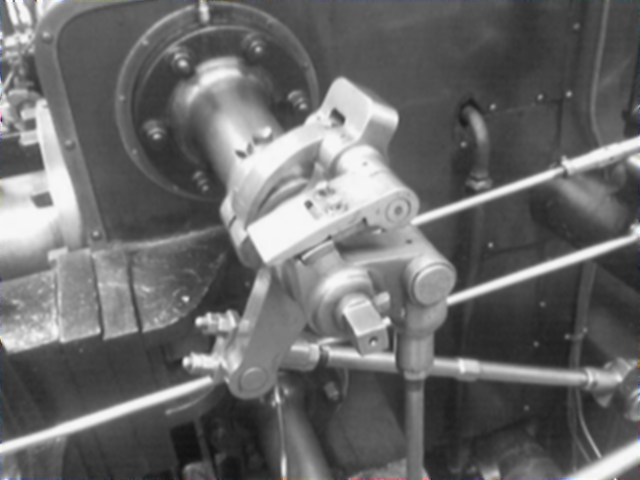
\includegraphics[width=0.9\textwidth]{images/canny-gaussian.png}
  \caption{Изображение после свертки с 5x5-фильтром Гаусса\label{canny-gaussian}}
\end{figure}

Вот пример 5x5 фильтра Гаусса, который используется для размытие изображения $A$, с $\sigma = 1,4$:
\begin{displaymath}
  B = \frac{1}{159}
  \begin{bmatrix}
    2 &  4 &  5 &  4 & 2 \\
    4 &  9 & 12 &  9 & 4 \\
    5 & 12 & 15 & 12 & 5 \\
    4 &  9 & 12 &  9 & 4 \\
    2 &  4 &  5 &  4 & 2
  \end{bmatrix} * A.
\end{displaymath}

\subsubsection{Нахождение градиента интенсивности изображения}
Край на изображении может быть расположен в различных направлениях, поэтому в операторе обнаружения краев Канни используются четыре фильтра для того, чтобы определять горизонтальные, вертикальные и диагональные края в размытом изображении. Каждые оператор обнаружения краев (например, перекрёстный оператор Робертса, Превитт или оператор Собеля) возвращает значения первой производной в горизонтальном направлении $G_y$ и вертикальном направлении $G_x$. Из них могут быть определены градиент и направление края:
\begin{gather*}
  G = \sqrt{G_x^2 + G_y^2},\\
  \Theta = \arctan{\frac{G_y}{G_x}}.
\end{gather*}

\begin{figure}
  \centering
  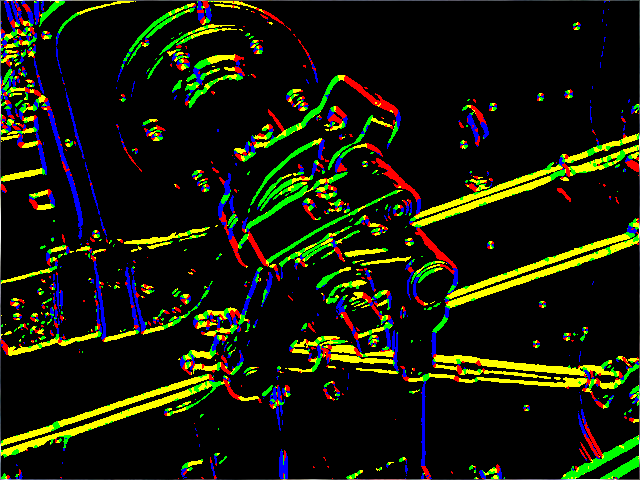
\includegraphics[width=0.9\textwidth]{images/canny-sobel.png}
  \caption{Бинарная карта краев, сделанная с помощью оператора Собеля с порогом равным $80$. Края разукрашены в зависимости от их направленности: желтый для $0^{\circ}$, синий для $90^{\circ}$, зеленый для $45^{\circ}$ и красный для $135^{\circ}$\label{canny-sobel}}
\end{figure}

Угол направленности округляется до одного из четырех значений, представляющих вертикальный, горизонтальный и два диагональных углы ($0$, $45$, $90$ и $135$ градусов, например).

\subsubsection{Подавление немаксимальных значений}
С учетом оценок градиетов изображения, поиск затем производится для определения предполагает ли величина градиента локальный максимум в его направлении. Например:
\begin{itemize}
  \item если округленный угол равен нулю, то предполагается, что точка находится на краю, если ее интенсивность больше, чем интенсивности в северном и южном направлениях;
  \item если округленный угол равен 90 градусам, то предполагается, что точка находится на краю, если ее интенсивность больше, чем интенсивности в западном и восточном направлениях;
  \item если округленный угол равен 135 градусам, то предполагается, что точка находится на краю, если ее интенсивность больше, чем интенсивности в северо-восточном и юго-западном направлениях;
  \item если округленный угол равен 45 градусам, то предполагается, что точка находится на краю, если ее интенсивность больше, чем интенсивности в северо-западном и юго-восточном направлениях.
\end{itemize}

\begin{figure}
  \centering
  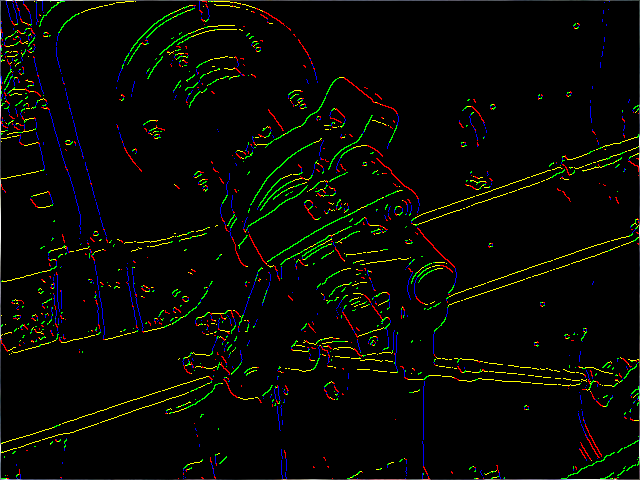
\includegraphics[width=0.8\textwidth]{images/canny-suppression.png}
  \caption{Та же самая бинарная карта, но уже после подавления немаксимальных значений. Края все еще разукрашены для обозначения направленности\label{canny-suppression}}
\end{figure}

На этом этапе мы имеем множество точек краев в форме \emph{бинарного} изображения.

\subsubsection{Отслеживание краев на изображении и определение порога}
Градиенты интенсивности, величина которых велика, вероятнее соответствуют краям на изображении по сравнению с теми, величина которых мала. В большинстве случаев невозможно установить порог (\emph{threshold}), который позволяет отличить край от не края. Поэтому Канни изпользовал установление порога с гистеризисом.

Установление порога с гистеризисом требует два порога --- высокий и низкий. Предположение, что края, представляющие интерес, должны представлять собой непрерывные кривые, позволяет не учитывать те пиксели, которые имеют высокие значения градиента, но не находятся на линии. Следовательно, мы начинаем с применения высокого порога. Это действие помечает края, которые с высокой степенью уверенности можно отнести к действительным. Используя информацию о направлениях, полученную ранее, края на изображении могут быть отслежены. Во время ослеживания края, мы применяем низкий порог, что позволяет отслеживать тусклые части краев, когда мы в состоянии найти начальную точку.

Как только это процесс завершен, мы имеем бинарное изображении, на котором каждый пиксель помечен как принадлежащий какому-либо краю или нет.

\begin{figure}
  \centering
  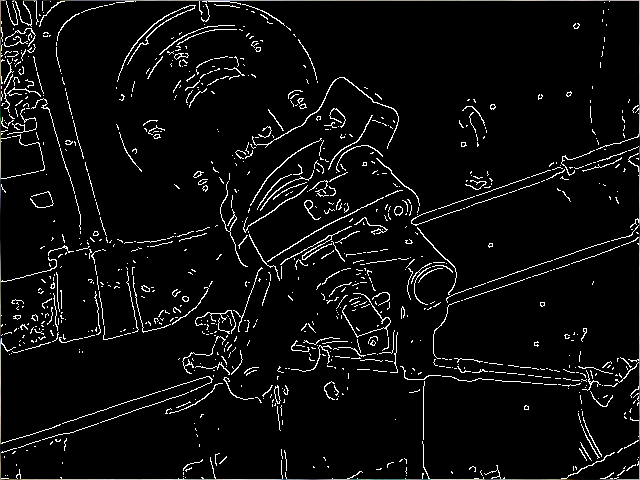
\includegraphics[width=0.8\textwidth]{images/canny-result.png}
  \caption{Изображение парового двигателя после применения оператора обнаружения краев Канни\label{canny-result}}
\end{figure}

\subsection{Параметры алгоритма}
В алгоритме Канни есть несколько регулируемых параметров, которые влияют на время вычислений и эффективность алгоритма.
\begin{itemize}
  \item Размер фильтра Гаусса: сглаживающий фильтр, используемый на первом этапе алгоритма, непосредственно влияет на результат детектора Канни. Меньшие фильтры меньше размывают изображение и позволяют определять мелкие, резкие края. Большие фильтры больше размывают изображение. Большие фильтры целесообразно использовать для определения больших, плавных краев, например, края радуги.
  \item Пороги: использование двух порогов с гистеризисом делает детектор более гибким, чем детекторы с одним пороговым значением. Но несмотря на это, общие проблемы пороговой классификации все еще имеют место быть. При слишком высоком пороге может быть утеряна важная информация. С другой стороны, при слишком низком пороге может быть ошибочно помечена несущественная информация, например, шум.
\end{itemize}

\subsection{Выводы}
Оператор обнаружения краев Канни легко приспосабливаем к различным условиям и требованиям. Его параметризация позволяет использовать его для распознавания краев различного характера.

\newpage

\section{Усиление простых классификаторов. Алгоритм AdaBoost}
Усиление простых классификаторов --- подход к решению задачи классификации путем комбинирования примитивных ``слабых'' (\emph{weak}) классификаторов в один ``сильный'' (\emph{strong}). Под ``силой'' классификатора в данном случае подразумевается эффективность (качество) решения задачи классификации. В данном разделе речь пойдет о семействе алгоритмов, в основе которых лежит алгоритм \emph{AdaBoost}, описанный в \cite{freund99}. Этот алгоритм был успешно использован во многих областях, в частности для задачи поиска лиц на изображении. Подход усиления простых классификаторов применяется во многих задачах и до сих пор является объектом множества как прикладных, так и теоретических исследований.

\subsection{Введение}
В основе метода усиления простых классификаторов лежит простая предпосылка: скомбинировать некоторое количество элементарных (простых) признаков таким образом, чтобы получить один, но более мощный. Классический пример: пусть человек, играющий на скачках, решил создать программу, которая бы предсказывала, придет ли интересующая его лошадь первой к финишу. Опросив некоторое количество играющих людей, он смог определить несколько эмпирических правил: ставь на лощадь, которая победила в трех предыдущих заездах, ставь на лощадь, ставки на которую максимальны и т.д. Ясно, что каждой из таких правил по отдельности недостаточно надежно и встает вопрос можно ли их оптимально скомбинировать для получения надежных результатов.

\subsection{AdaBoost}
Мы рассмотрим один из самых ранних алгоритмов из данного семейства --- AdaBoost. Этот алгоритм был опубликован в 1996 году и послужил основой для всех последующих исследований в данной области. На его основе была построена на данных момент, пожалуй, самая эффективная (как по уровню распознавания, так и по скорости работы) система поиска объектов на изображении \cite{viola01}. На данный момент наиболее распростаненными вариантами базового алгоритма являются \emph{Gentle AdaBoost} и \emph{Real AdaBoost}, превосходящие базовый алгоритм по своим характеристикам, но сохраняющие все основные принципы. К основным достоинствам \emph{AdaBoost} и его вариантов можно отнести высокую скорость работы, высокую эффективность распознавания, простоту реализации, общность.

\subsubsection{Описание алгоритма}
Требуется построить классифицирующую функцию $F : X \to Y$, где $X$ --- пространство векторов признаков, $Y$ --- пространство меток классов. Пусть в нашем распоряжении имеется обучающая выборка $(x_1, y_1), \dots, (x_M, y_M)$, где $x_i \in X$ --- вектор признаков, а $y_i \in Y$ --- метка класса, к которому принадлежит $x_i$. Для простоты изложения мы будем рассматривать задачу с двумя классами, то есть $Y = \{-1; +1\}$. Также у нас есть семейство простых классифицирующих функций $H: X \to Y$. Мы будем строить финальный классификатор в следующей форме:
\begin{displaymath}
  F(x) = \sign{\sum_{t = 1}^T{\alpha_th_t(x)}},
\end{displaymath}
где $\alpha_t \in R, h_t \in H.$ Построим итеративный процесс, где на каждом шаге будем добавлять новое слагаемое:
\begin{displaymath}
  f_t(x) = \alpha_th_t(x),
\end{displaymath}
вычисляя его с учетом работы уже построенной части классификатора.

\begin{algorithm}
  \caption{Алгоритм AdaBoost}
  \label{adaboost-algorithm}
  \begin{enumerate}
  \item Пусть $(x_1, y_1), \dots, (x_M, y_M)$ --- обучающая выборка и $D_1(i) = \frac{1}{M}$ --- начальное распределение.
  \item Для каждого шага $t = 1,2,..,T$:
    \begin{enumerate}
      \item Тренируем слабый классификатор, используя распределение $D_t$.
      \item Получаем слабый классификатор $h_t(x) \in H$ с ошибкой классификации:
        \begin{displaymath}
          \epsilon_t = \sum_{i = 1}^M{D_t(i) \cdot (h_t(x_i) \neq y_i)}).
        \end{displaymath}
      \item Вычисляем коэффициент $\alpha_t = \frac{1}{2}\ln{\frac{1 - \epsilon_t}{\epsilon_t}}$.
      \item Обновляем:
        \begin{displaymath}
          D_{t + 1}(i) = \frac{D_t(i)\exp{(-\alpha_ty_ih_t(x_i))}}{Z_t},
        \end{displaymath}
        где $Z_t$ --- нормализующий делитель, такой что $D_{t + 1}$ будет распределением.
    \end{enumerate}
  \item Составляем сильный классификатор следующим образом:
    \begin{displaymath}
      F(x) = \sign{\sum_{t = 1}^T{\alpha_th_t(x)}}.
    \end{displaymath}
  \end{enumerate}
\end{algorithm}

На каждом шаге будем для каждого примера $(x_i, y_i)$ из обучающей выборки вычислять его ``вес''. Положим $D_1(i) = \frac{1}{M}$, тогда
\begin{displaymath}
  D_{t + 1}(i) = \frac{D_t(i)\exp{(-y_if_t(x_i))}}{Z_t},
\end{displaymath}
где $Z_t$ --- нормализующий коэффициент, такой что
\begin{displaymath}
  \sum_{i = 1}^M{D_{t + 1}(i)} = 1.
\end{displaymath}

Вес каждого элемента обучающей выборки на текущем шаге задает ``важность'' этого примера для очередного шага обучения алгоритма. Чем больше вес, тем больше алгоритм будет ``стараться'' на данном шаге классифицировать этот пример правильно. Как видно из формулы, чем уверенней пример распознается предыдущими шагами, тем его вес меньше; таким образом, самые большие веса получают примеры, которые предыдущими шагами были классифицированы неверно. Иначе говоря, мы варьируем веса таким образом, чтобы классификатор, включенный в комитет на текущем шаге, ``концентрировался'' на примерах,  с которыми предыдущие шаги ``не справились''. Таким образом на каждом шаге мы работаем с какой-то частью данных, плохо классифицируемой предыдущими шагами, а в итоге комбинируем все промежуточные результаты.

Очередной простой классификатор мы будем выбирать, исходя из взвешенной с распределением $D_t$ ошибки. Мы выбираем (тренируем) $h_t \in H$, минимизирующий взвешенную ошибку классификации
\begin{displaymath}
  \epsilon_t = \sum_{i = 1}^M{D_t(i) \cdot (h_t(x_i) \neq y_i)}.
\end{displaymath}

Заметим, что если рассмотреть $D_t$ как распределение вероятности над $X$, что правомерно, так как
\begin{displaymath}
  \sum_{i = 1}^M{D_{t + 1}(i)} = 1,
\end{displaymath}
то
\begin{displaymath}
  \epsilon_t = \underset{x \sim D_t}{\Pr}(h_t(x) \neq y).
\end{displaymath}

Далее вычисляется вклад текущего слагаемого классифицирующей функции
\begin{displaymath}
  \alpha_t = \frac{1}{2}\ln{\frac{1 - \epsilon_t}{\epsilon_t}}.
\end{displaymath}

Мы продолжаем процесс до некоторого шага $T$, номер которого определяется вручную.

\subsubsection{Роль простого классификатора}
В этом разделе мы уделим внимание фундаменту всех методов усиления простых классификаторов --- семейству простых классификаторов $H : X \to Y$.

Для ясности приведем пример. Пусть входные данные --- это $n$-мерные вектора $x \in R^n$, тогда
\begin{displaymath}
  H = h^{\Theta, k}(x = (x_1, \dots, x_k, \dots, x_n)) = \begin{cases}+1, x_k > \Theta,\\ -1, x_k < \Theta\end{cases},
\end{displaymath}
то есть это порог по $k$-той координате.

Как при таком множестве $H$ происходит выбор наилучшего классификатора $h^{\Theta, k}$ на каждой итерации? В данном случае делается следующее: для каждого $k = 1..n$ вычисляется порог $\Theta'_k$, реализующий минимум взвешенной ошибки $\epsilon_t$, затем из полученных классификаторов $h^{\Theta, k}, k = 1..n$ выбирается соответствующий минимальной $\epsilon_t$.

Несмотря на свою простоту, этот классификатор, усиленный алгоритмом \emph{AdaBoost}, дает весьма впечатляющий результаты. Система поиска объектов на изображении \cite{viola01} находит $95\%$ всех искомых объектов с $0,0001\%$ ложных срабатываний.

Какими свойствами должен обладать простой классификатор? В первую очередь, вероятность его ошибки должна быть хотя бы немного меньше $^1/_2$, то есть он должен работать лучше, чем ``подбрасывание монеты'':
\begin{displaymath}
  \exists \gamma > 0: \underset{x \sim D_m}{\Pr}(h(x) \neq y) \leq \frac{1}{2} - \gamma.
\end{displaymath}

Также простой классификатор должен быть максимально простой структуры (обладать малой $VC$-размерностью). Это связано с оценкой ошибки обобщения сильного классификатора.

Самыми часто используемыми на практике простыми классификаторами являются пороги (\emph{stumps}) и \emph{CART} решающие деревья.

\subsubsection{Внутреняя механика AdaBoost}

В этом разделе мы попытаемся пролить немного света на внутреннюю механику алгоритма. Фактически, \emph{AdaBoost} осуществляет два действия:
\begin{itemize}
  \item отбор простых классификаторов (простых признаков);
  \item комбинирование отобранных классификаторов.
\end{itemize}

Первое действие является своеобразным отображением пространства входных векторов в пространство значений простых классификаторов:
\begin{displaymath}
  x = (x_1, x_2, \dots, x_N) \to (h_1(x), h_2(x), \dots, h_M(x)).
\end{displaymath}

Комбинирование простых классификаторов происходит линейно (составляется линейная комбинация), а решение принимается в зависимости от знака полученной комбинации. Это фактически эквивалентно разделению пространства значений простых классификаторов гиперплоскостью и принятие решения в зависимости от того, по какую сторону гиперплоскости лежит отображение вектора признаков.

Таким образом, готовый классификатор производит вначале отображение в некое пространство, обычно намного более высокой размерности, чем исходное, в котором производит линейную классификацию. На этапе тренировки алгоритм последовательно строит и это отображение, и саму гиперплоскость.

Стоит заметить, что работа \emph{AdaBoost} в значительной мере напоминает работу алгоритма ядерной машины опорных векторов (\emph{Kernel Support Vector Machine}).

Одна из интерпретаций работы алгоритмов на основе \emph{AdaBoost} основана на понятии ``грани'' (\emph{margin}). В случае \emph{AdaBoost} грань определяется как:
\begin{displaymath}
  \mu(x, y) = \frac{\sum_{m = 1}^M{y \cdot f_m(x)}}{\sum_{m = 1}^M{\alpha_m}}.
\end{displaymath}

Эту величину можно интерпретировать как меру ``уверенности'' классификатора в примере $(x, y)$. Если классификация правильная, то грань больше нуля, иначе грань отрицательна. Чем больше простых классификаторов правильно классифицируют пример, тем больше грань.

Если учесть то, как на каждом шаге вычисляются веса примеров, то легко видеть, что на каждом шаге \emph{AdaBoost} пытается максимизировать минимальную грань тренировочной выборки. Утверждается, что данное дейтсвие положительно сказывается на обобщающих способностях алгоритма. Больше про данную интерпретацию семейства алгоритмов на основе \emph{AdaBoost} можно прочитать в \cite{rosset04}.

Для более детального знакомства предлагаем обратиться к указанной в библиографии литературе, а также посетить сайт \url{http://www.boosting.org}.

\newpage


\section{Охрана труда, экологическая безопасность, энергосбережение. Реализация пространственно-антропометрической эргономической совместимости работника при разработке методов распознования, захвата и сопровождения движущихся объектов}

\subsection{Пространственно-антропометрическая эргономическая совместимость и ее сущность}
\emph{Эргономика} --- это научная дисциплина, комплексно изучающая человека в конкретных условиях его деятельности в современном производстве. Основной объект исследования эргономики --- \emph{система ``человек--машина''}. Эргономические исследования и разработки заключаются в изучении человеко-машинных систем, а именно в исследовании характеристик человека, машины, окружающей среды, характера взаимодействия этих компонентов в конкретных условиях и организации производственной зоны, создании рабочих мест, машин, пультов управления, обеспечивающих максимальное удобство для человека, оптимальные условия взаимодействия с машиной и объектом управления.\cite{devisilov09}

На человека в процессе труда действует множество факторов: вид трудовой деятельности, ее тяжесть и напряженность, условия, в которой она осуществляется (вредный вещества, излучения, климатические условия, освещенность и т.д.), психофизиологические возможности человека (прежде всего антропометрические характеристика человека, скорость реакций на различные раздражители, особенности воприятия человеком цвета и т.д.). Для того чтобы человеко-машинная система функционировала эффективно и не приносила ушерба здоровью человека, необходимо прежде всего обеспечить совместимость характеристик машины и человека. Совместимость человека с машиной определяется его антропометрической, сенсомоторной, энергетической (биомеханической) и психофизиологической совместимостью.\cite{devisilov09}

Нас прежде всего интересует антропометрическая совместимость.

\emph{Антропометрическая совместимость} предполагает учет размеров тела человека, возможность обзора внешнего пространства, положения (позы) оператора в процессе работы при создании рабочего места.\cite{devisilov09}

Например, на рис.~\ref{access-zones} показаны антропометрические зоны досягаемости рук человека в положении стоя.

\begin{figure}
  \centering
  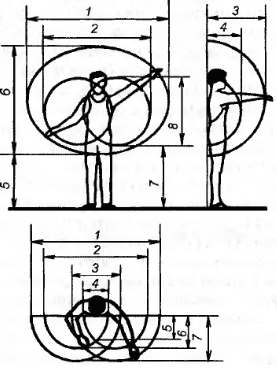
\includegraphics[width=0.4\textwidth]{images/devisilov-6-6}
  \caption{Зоны досягаемости рук человека в положении стоя в вертикальной и горизонтальной плоскостях: 1--8 --- номера зон\label{access-zones}}
\end{figure}

К антропометрическим характеристикам человека относятся статические характеристики --- размеры тела человека и его отдельных частей (головы, ног, рук, кистей, стоп, ширина плеч, таза и т.п.) и динамические характеристики -- возможные углы поворота отдельных частей тела, зоны досягаемости.\cite{devisilov09}

\begin{figure}
  \centering
  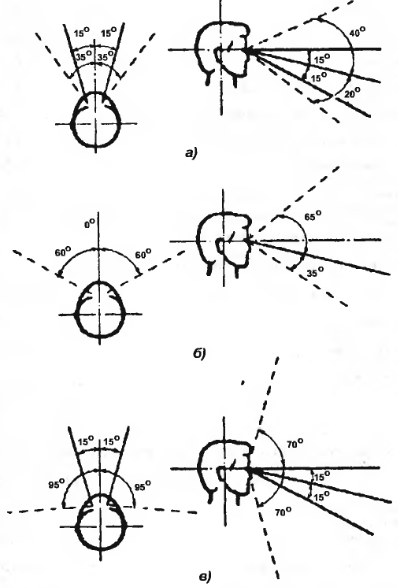
\includegraphics[width=0.75\textwidth]{images/devisilov-6-7}
  \caption{Информационные зоны визуального поля: а --- при повороте глаз; б --- при повороте головы; в --- при повороте головы и глаз; --- ---- оптимальные углы обзора; - - - --- максимальные углы обзора\label{visual-zones}}
\end{figure}

Информационные зоны визуального поля обзора человека представлены на рис.~\ref{visual-zones} и определяются полями зрения (поле ясного зрения, поле обзора и т.д.), размеры которых выражаются углами зрения.\cite{devisilov09}

\subsection{Трудовая функция работника, характеристика трудового процесса}
Характер и организация трудовой деятельности оказывают существенное влияние на изменение функционального состояния организма человека. Многообразные формы трудовой деятельности делятся на физический и умственный труд.\cite{belov09}

\emph{Физический труд} характеризуется нагрузкой на опорно-двигательный аппарат и функциональные системы организма человека (сердечно-сосудистую, нервно-мышечную, дыхательную и др.), обеспечивающие его деятельность.\cite{belov09}

\emph{Умственный труд} объединяет работы, связанные с приемом и переработкой информации, требующей преимущественного напряжения сенсорного аппарата, внимания, памяти, а также активизации процессов мышления, эмоциональной сферы. Для данного вида труда характерна \emph{гипокинезия}, т.е. значительное снижение двигательной активности человека, приводящее к ухудшению реактивности организма и повышению эмоционального напряжения. Гипокинезия является одним из условий формирования сердечно-сосудистой патологии у лиц умственного труда. Длительная умственная нагрузка оказывает угнетающее влияние на психическую деятельность: ухудшаются функции внимания (объем, концентрация, переключение), памяти (кратковременной и долговременной), восприятия (появляется большое число ошибок).\cite{belov09}

Труд программиста является умственным (интеллектуальным). Более того он относится к наиболее сложной форме трудовой деятельности, требующей значительного объема памяти, напряжения, внимания, --- \emph{творческому труду}. Труд программистов приводит к значительному повышению нервно-эмоционального напряжения. При таком напряжении, связанном с умственной деятельностью, можно наблюдать тахикардию, повышение кровяного давления, увеличение легочной вентиляции и потребления кислорода, повышение температуры тела и другие изменения со стороны вегетативных функций человека.\cite{belov09}

Тяжесть и напряженность труда характеризуется степенью функциональнго напряжения организма. Оно может быть энергетическим, зависящим от мощности работы --- при физическом труде, и эмоциональным --- при умственным труде, когда имеет место информационная перегрузка.\cite{belov09}

Однообразие выполняемых операций приводит к определенному техническому состоянию человека, называемому \emph{монотомией}. Признаком монотомии является либо перегрузка одинаковой информацией, либо недостаток новой. Это накладывает отпечаток на функциональное состояние человека: он теряет интерес к выполняемой работе. Для него рабочее время как бы остановилось, и он с нетерпением джет окончания смены, его клонит ко сну. Монотонная работа снижает эффективность труда.\cite{belov09}

Физическая тяжесть труда программиста находится на минимальном уровне (программисту не надо поднимать грузы, делать частые наклоны и т.д.).
Чего нельзя сказать про напряженность труда.\cite{belov09}

\emph{Напряженность труда} характеризуется эмоциональной нагрузкой на организм при труде, требующем преимущественно интенсивной работы мозга по получению и переработке информации.\cite{belov09}

Программисту приходится работать с монитором более 4 ч. Деятельность программиста является творческой (эвристической) деятельностью, которая требует решения сложных задач при отсутствии очевидного алгоритма решения. Согласно \cite{belov09}, ее следует отнести к напряженному труду 2-й степени тяжести.

\subsection{Реализация требований пространственно-антропометрической совместимости и проектирование рабочего места в соответствии с ними}
Организация рабочего места, конструкция органов контроля и управления должны учитывать антропометрические характеристики человека.\cite{devisilov09}

Оптимальное расположение и компоновка рабочего места, обеспечение удобной позы и свободы трудовых движений, использование оборудования, отвечающего требованиям эргономики и инженерной психологии, обеспечивают наиболее эффективный трудовой процесс, уменьшают утомляемость и предотвращают опасность возникновения профессиональных заболеваний.

Оптимальная поза человека в процессе трудовой деятельности обеспечивает высокую работоспособность и производительность труда. Неправильное положение тела на рабочем месте приводит к быстрому возникновению статической усталости, снижению качества и скорости выполняемой работы, а также к снижению реакции на опасности. Нормальной рабочей позой следует считать такую, при которой работнику не требуется наклоняться вперед больше, чем на \(10\dots15^{\circ}\); наклоны назад и в стороны нежелательны; основное требование к рабочей позе --- прямая осанка.

Работа в позе сидя более рациональна и менее утомительна, так как уменьшается высота центра тяжести над площадью опоры, повышается устойчивать тела, снижается напряжение мышц, уменьшается нагрузка на сердечно-сосудистую систему. В положении сидя обеспечивается возможность выполнять работу, требующую точность движения. Однако и в этом случае могут возникать застойные явления в органах таза, затруднение работы органов кровообращения и дыхания.

Смена позы приводит приводит к перераспределению нагрузки на группы мыщц, улучшению условий кровообращения, ограничивает монотонность. Поэтому, где это совместимо с технологией и условиями производства, необходимо предусматривать выполнение работы как стоя, так и сидя, с тем чтобы рабочие по своему усмотрению могли изменять положение тела.

\begin{figure}
  \centering
  \subfloat[][Зоны для выполнения ручных операций и размещения органов управления: 1 --- зона для размещения наиболее важных и очень часто используемых органов управления (оптимальная зона моторного поля); 2 --- зона для размещения часто используемых органов управления (зона легкой досягаемости моторного поля); 3 --- зона для размещения редко используемых органов управления (зона досягаемости моторного поля)]{\label{hand-operation-zones}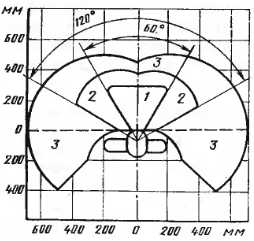
\includegraphics[width=0.4\textwidth]{images/devisilov-6-8}}
  \qquad
  \subfloat[][Зоны для выполнения ручных операций и размещения органов управления в вертикальной плоскости: 1 --- зона для размещения очень часто используемых и наиболее важных органов управления (оптимальная зона моторного поля); 2 --- зона для размещения часто используемых органов управления (зона легкой досягаемости моторного поля); 3 --- зона для размещения редко используемых органов управления (зона досягаемости моторного поля)]{\label{vertical-hand-operation-zones}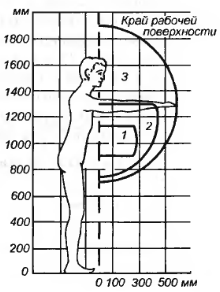
\includegraphics[width=0.4\textwidth]{images/devisilov-6-9}}
  \caption{}
\end{figure}

Пространство рабочего места, в котором осуществляются трудовые процессы, должно быть разделено на рабочие зоны. Зонирование рабочего места в горизонтальной и вертикальной плоскостях представлено на рис.~\ref{hand-operation-zones},~\ref{vertical-hand-operation-zones}. Рабочую зону, удобную для действия обеих рук, нужно обязательно совмещать с зоной визуального обзора.\cite{devisilov09}

Важное эргономическое значение имеет рабочая поза человека. Рабочая поза ``стоя'' требует больших энергетических затрат и приводит к быстрому утомлению. Рабочая поза ``сидя'' менее утомительно, и она более предпочтительно. Рабочая зона должна быть организована так, а органы управления должны быть так расположены, чтобы в рабочей позе проекция центра тяжести тела человека была расположена в пределах площади его опоры. В противном случае положение тела человека будет неустойчивым и потребует значительных мышечных усилий. Это может привести к заболеваниям опорно-двигательного аппарата (например, искривление позвоночника), быстрому утомлению, травме.\cite{devisilov09}

Составной частью рабочего места в положении ``сидя'' является рабочее кресло оператора. Кресло должно соответствовать антропометрическим данным человека. Основные геометрические параметры рабочих кресел стандартизованы. Целесообразно применять кресла с регулируемыми параметрами (высотой, углом, наклона спинки), чтобы приспособить их под антропометрические характеристики конкретного человека.\cite{devisilov09}

Устройства визуальной информации оператора в зависимости от частоты их использования также должны располагаться в соответствующих зонах визуального поля человека. При частом использовании приборы должны располагаться в пределах оптимальных углов обзора, при редком --- в пределах максимальных углов обзора.\cite{devisilov09}

\begin{figure}
  \centering
  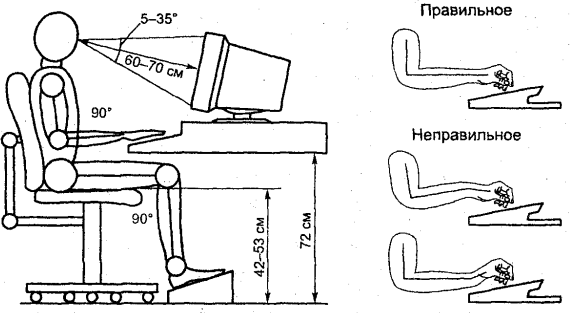
\includegraphics[width=0.9\textwidth]{images/mihnuk-3-14}
  \caption{Правильная позиция оператора и положение его рук при работе на клавиатуре\label{operator-position}}
\end{figure}

Уровень глаз при вертикальном расположенном экране видеодисплея должен приходиться на центр или \(^2/_3\) высоты экрана. Линия взора должна быть перпендикулярна к центру экрана. При работе на клавиатуре необходимо соблюдать правильное положение рук оператора (рис~\ref{operator-position}).\cite{mihnuk07}

Расположение рабочих мест для пользователей видеодисплеев и ПЭВМ в подвальных помещениях не допускается.\cite{mihnuk07}

Площадь на одно рабочее место с видеодисплеем и ПЭВМ должна составлять не менее \(6,0 \text{м}^2\), а объем --- не менее \(20,0 \text{м}^3\).\cite{mihnuk07}

При размещении рабочих мест расстояние между рабочими столами должно быть не менее \(2,0 \text{м}\), а расстояние между боковыми поверхностями видеомониторов --- не менее \(1,2 \text{м}\). Рабочие места сотрудников, выполняющих творческую работу и требующей значительного умственного напряжения или высокой концентрации внимания, рекомендуется изолироваться друг от друга перегородками высотой от \(1,5 \text{м}\).\cite{mihnuk07}

Рабочие столы следует размещать таким образом, чтобы мониторы были ориентированы боковой стороной к световым проемам, чтобы естественный свет падал преимущественно слева.
\newpage

\section{Технико-экономическое обоснование}

\subsection{Характеристика проекта}
Немного о проекте, для кого может представлять интерес.

\subsection{Расчет экономического эффекта у разработчика}

\subsection{Расчет экономического эффекта у пользователя}

\section*{ЗАКЛЮЧЕНИЕ}
\addcontentsline{toc}{section}{Заключение}

В этом разделе была описан обобщенная модель для захвата и оценки позы объектов со сложной конфигурацией (detection and articulated pose estimation of not-rigid objects). Как утверждается в \cite{andriluka09}, вышеописанный метод превосходит другие современные модели, разработанные для узкоспециализированных задач, но при этом оставаясь на удивленье очень простым. Причинами этого превосходного результата является комбинация двух компонентов: строго дифференцирующей модели внешних признаков и гибкая модель априорной вероятности конфигураций частей объекта.

\newpage

\begin{thebibliography}{99}

\bibitem{forsight04}
  Д. Форсайт, Ж. Понс,
  \emph{Компьютерное зрение. Современный подход}.
  М.: Издательский дом ``Вильямс'',
  2004.

\bibitem{shapiro06}
  Л. Шапиро, Дж. Стокман,
  \emph{Компьютерное зрение}.
  М.: БИНОМ. Лаборатория знаний,
  2006.

\bibitem{andriluka09}
  M. Andriluka, S. Roth, B. Schiele,
  \emph{Pictorial structures revisited: people detection and articulated pose estimation}.
  IEEE Conference on Computer Vision and Pattern Recognition,
  2009.

\bibitem{andriluka08}
  M. Andriluka, S. Roth, B. Schiele,
  \emph{People-tracking-by-detection and people-detection-by-tracking}.
  IEEE Conference on Computer Vision and Pattern Recognition,
  2008.

\bibitem{belongie02}
  S. Belongie, J. Malik, J. Puzicha,
  \emph{Shape matching and object recognition using shape contexts}.
  IEEE Transactions on Pattern Analysis and Machine Intelligence,
  2002.

\bibitem{belongie00}
  S. Belongie, J. Malik, J. Puzicha,
  \emph{Shape context: a new descriptor for shape matching and object recognition}.
  Conference on Neural Information Processing Systems,
  2000.

\bibitem{felzenszwalb05}
  P.F. Felzenszwalb, D.P. Huttenlocher,
  \emph{Pitorial structures for object recognition}.
  International Journal of Computer Vision,
  2005.

\bibitem{freund99}
  Y. Freund, R.E. Schapire,
  \emph{A Short Introduction to Boosting}.
  Journal of Japanese Society for Artificial Intelligence, 14(5):771--780, September,
  1999.

\bibitem{viola01}
  P. Viola, M. Jones,
  \emph{Robust Real-time Object Detection}.
  In Proc. 2nd Int'l Workshop on Statistical and Computational Theories of Vision --- Modeling, Learning, Computing and Sampling, Vancouver, Canada,
  July 2001.

\bibitem{rosset04}
  Rosset, Zhu and Hastie,
  \emph{Boosting as a Regularized Path to a Maximum Margin Classifier}.
  Journal of Machine Learning Research 5 (2004) 941-973,
  2004.

\bibitem{canny86}
  J. Canny,
  \emph{A Computational Approach To Edge Detection}.
  IEEE Transactions on Pattern Analysis and Machine Intelligence, 8(6):679–714,
  1986.

\bibitem{deriche87}
  R. Deriche,
  \emph{Using Canny's criteria to derive a recursively implemented optimal edge detector}.
  International Journal of Computer Vision, Vol. 1, pp. 167–187,
  April 1987

\bibitem{lindeberg98}
  T. Lindeberg,
  \emph{Edge detection and ridge detection with automatic scale selection}.
  International Journal of Computer Vision, 30, 2, pp 117—154,
  1998.

\bibitem{mihnuk07}
  Михнюк Т.Ф.,
  \emph{Охрана труда и основы экологии}.
  Минск: ``Вышэйшая школа'',
  2007.

\bibitem{devisilov09}
  Девисилов В.А.,
  \emph{Охрана труда}.
  М.: ФОРУМ,
  2009.

\bibitem{belov09}
  Белов С.В.,
  \emph{Безопасность жизнедеятельности}.
  М.: Высшая школа,
  2007.

\bibitem{decree432}
  Указ Президента РБ №432 от 31 августа 2009 года,
  \emph{О некоторых вопросах приобретения имущественных прав на результаты научно-технической деятельности и распоряжения этими правами}.
  \href{http://president.gov.by/press76885.html}{http://president.gov.by/press76885.html}.

\bibitem{palitsyn06}
  Палицын В.А.,
  \emph{Технико-экономическое обоснование дипломных проектов. В 4-х частях. Часть 4: проекты программного обеспечения}.
  Мн.: БГУИР,
  2006.

\end{thebibliography}


\end{document}
